%!TEX ROOT=formularioFisica.tex

\section{Circuiti elettrici}\label{sec:circElettr}
Questa sezione è strettamente legata alla precedente ma, vista l'importanza ne merita una sua.\\
I circuiti elettrici sono usati ovunque nel mondo d'oggi e hanno una simbologia tutta loro. Di 
seguito verranno riportati i principali elementi circuitali e il loro funzionamento con le relative
formule.

\subsection{Elementi circuitali}

\subsubsection{Generatori}
Ci sono due tipi di correnti e di conseguenza due tipi di generatori. Nelle successive parti, si
divideranno i circuiti principali in base al tipo di corrente presente.\\
I generatori producono tutti una certa \textbf{Differenza di potenziale} o d.d.p.\ nel circuito.
Questa d.d.p. è regolata dalla legge di Ohm (vedi pagina~\pageref{par:circElettr:elem:res:ohm}). 
In genere la
lettera che denota un generatore di differenza di potenziale è o $V$ (dall'unità di misura, Volt),
o $\mathcal{E}$. Vi è grande differenza soltanto tra generatori \textbf{reali} in cui
è presente una resistenza interna, quindi si ha che
\begin{equation*}
  \mathcal{E} = \overbrace{Ri}^{V} + ri
\end{equation*}
$R$: resistenza totale degli elementi circuitali\\
$r$: resistenza interna\\ [\baselineskip]
Generalmente la $\mathcal{E}$ viene anche definita \textbf{forza elettromotrice}.\\
Il suo valore può anche essere definito in funzione del lavoro ($L$) che il generatore deve
fare per spostare una carica ($q$) da un polo all'altro
\begin{equation*}
  \mathcal{E} = \frac{L}{q}
\end{equation*}

\paragraph{Continua}
La corrente generata da questi generatori è corrente \textbf{continua}, ovvero che mantiene il
verso nel tempo. Il simbolo utilizzato piu frequentemente è
\begin{center}
  \begin{circuitikz}
    \draw(0,0) to[battery1,v>=9<\volt>] (2,0);
  \end{circuitikz}
\end{center}
Il polo positivo è quello più grande e la corrente va da $+$ a $-$.

\paragraph{Alternata}
La corrente generata da questi generatori è corrente \textbf{alternata}, ovvero non ha un verso
e cambia intensità istante per istante in modo sinusoidale. Il simbolo più usato è
\begin{center}
  \begin{circuitikz}
    \draw(0,0) to[sV, l=9<\volt>] (2,0);
  \end{circuitikz}
\end{center}

\subsubsection{Resistenze}
Le resistenze sono uno degli elementi fondamentali dei circuiti elettrici. Esse oppongono 
resistenza alla corrente che le attraversa, permettendo quindi una tensione minore per un specifico
elemento. La loro unità di misura è l'Ohm ($\Omega$).\\
Il loro simbolo è
\begin{center}
  \begin{circuitikz}
    \draw(0,0) to[R, l=10<\kilo\ohm>] (2,0);
  \end{circuitikz}
\end{center}

\paragraph{Leggi di Ohm}\label{par:circElettr:elem:res:ohm}
Le leggi di Ohm mettono in definiscono la differenza di potenziale e le caratteristiche fisiche di 
una resistenza.

\begin{alignat*}{2}
  R &= \frac{\Delta V}{i} &\qquad R &= \rho\frac{l}{S}
\end{alignat*}
La prima mette in relazione la ddp e la corrente con la resistenza.\\
La seconda mette in relazione la resistività ($\rho$), la lunghezza del corpo ($l$) e la sezione 
($S$) con la resistenza.

\subsubsection{Condensatori}
Un condensatore è composto da due \emph{armature} che hanno cariche di segno opposto, una positiva
e l'altra negativa. Il compito di un condensatore all'interno di un circuito è di immagazzinare 
carica e rilasciarla. Viene usato ad esempio nei flash delle macchine fotografiche dove viene
rilasciata in un attimo la carica immagazzinata in un certo tempo.\\
La loro unità di misura è il Farad (F).\\
Il loro simbolo è
\begin{center}
  \begin{circuitikz}
    \draw(0,0) to[C=1<\micro\farad>] (2,0);
  \end{circuitikz}
\end{center}
La capacità di un condensatore è regolata dalle formule descritte a 
pagina~\pageref{sub:elettrostatica:capacita}.

\subsubsection{Induttanza}
L'induttanza è strettamente collegata al fenomeno dell'auto induzione, che è strettamente legato
alla \hyperref[subsec:mag:fnl]{Legge di Faraday-Neuman-Lenz}. Per capirla, prendiamo come
esempio il seguente circuito
\begin{center}
  \begin{circuitikz}\ctikzset{bipoles/length=.8cm}
    \draw 
    (0,0) 
    to[battery1] (1,0)
    to[switch] (2,0)
    to[R] (2,1)
    to[short] (0,1)
    to[short] (0,0);
  \end{circuitikz}
\end{center}
Per la legge di Biot-Savart, si genererà un campo magnetico quando si chiude il circuito e scorrerà
della corrente. Per la Legge di Faraday-Neuman-Lenz (pag.~\pageref{subsec:mag:fnl}) 
la variazione di campo magnetico produrrà una corrente indotta all'interno di questo circuito che 
si oppone alla corrente nel momento della carica e la favorisce nella scarica. Questo ci porta all'
introduzione di un nuovo elemento circuitale: l'induttanza
\begin{center}
  \begin{circuitikz}
    \draw(0,0) to[L] (2,0);
  \end{circuitikz}
\end{center}
Il flusso del cicuito è proporzionale alla corrente per la legge di Faraday-Neuman-Lenz. Quindi
possiamo scrivere
\begin{equation*}
  \Phi(\vec{B}) = L\cdot i
\end{equation*}
dove $L$ è la nostra induttanza che dipenda da circuito a circuito.\\
Se ora usiamo la nuova definizione di flusso possiamo scrivere
\begin{equation*}
  \mathcal{E} = -\der{\Phi(\vec{B})}{t} = -\der{(Li)}{t} = 
  -L\der{i}{t} 
\end{equation*}
Cosa ci dice questo? Che se $\der{i}{t}\neq0$ allora $\mathcal{E}_{ind}\neq0$, se invece
$\der{i}{t}=0$, allora $i(t)=\text{costante}$.\\
Essendo l'elemento dell'induttanza un solenoide, possiamo isolare $L$ e scrivere
\begin{equation*}
  L = \frac{\Phi(\vec{B})}{i} = \frac{N\mu\frac{Ni}{l}S}{i} = \mu\frac{N^2S}{l}
\end{equation*}
dove $\mu$ è la permeabilità magnetica che può essere assoluta (\hyperref[tab:mu0]{$\mu_0$}) o
relativa ($\mu_r\mu_0$), $N$ il numero di spire, $S$ la superficie e $l$ la lunghezza del 
solenoide. L'unità di misura è l'\textit{Henry} (H).

\subsubsection{Interruttore}
L'interruttore permette di interrompere il flusso di carica, ovvero di aprire o chiudere il 
circuito. Il suo simbolo è
\begin{center}
  \begin{circuitikz}
    \draw(0,0) to[switch] (2,0);
  \end{circuitikz}
\end{center}


\subsection{Corrente elettrica}
La corrente elettrica è frutto di una d.d.p.\ applicata in un circuito. Essa, per definizione è
\begin{equation*}
  i = \frac{\Delta q}{\Delta t} = \der{q(t)}{t}
\end{equation*}

\subsection{Collegamenti}
Ci sono 2 tipi di collegamenti: \textbf{in serie} ed \textbf{in parallelo}.\\
Se due componenti sono in serie, la stessa corrente $i$ li attraversa e sono posti uno dietro 
l'altro. Se sono in parallelo invece la corrente si divide, mantenendo costante la d.d.p.

\subsubsection{Capacità equivalente di condensatori in \emph{serie}}
\begin{center}
  \begin{circuitikz}
    \draw
    (0,0)
    to [short] (1,0)
    to [C=$C_1$] (2,0)
    to [short] (3,0)
    to [C=$C_2$] (4,0)
    to [short] (5,0);
  \end{circuitikz}
\end{center}
Questo ``circuito'' può essere ridotto ad un solo condensatore la cui capacità deve essere
\begin{equation*}
  \frac{1}{C_e} = \frac{1}{C_1} + \frac{1}{C_2}
\end{equation*}

\subsubsection{Capacità equivalente di condensatori in \emph{parallelo}}
\begin{center}
  \begin{circuitikz}
    \draw 
    (-1,0)
    to [short, o-] (0,0)
    to [short, *-] (0,1)
    to [short] (1,1)
    to [C=$C_1$] (2,1)
    to [short] (3,1)
    to [short] (3,0)

    (0,0) 
    to [short, *-] (0,-1)
    to [short] (1,-1)
    to [C=$C_2$] (2,-1)
    to [short] (3,-1)
    to [short] (3,0)

    (3,0)
    to [short, *-o] (4,0);
  \end{circuitikz}
\end{center}
Questo ``circuito'' può essere ridotto ad un solo condensatore la cui capacità deve essere
\begin{equation*}
  C_e = C_1 + C_2
\end{equation*}

\subsubsection{Proprietà di condensatori in serie ed in parallelo}
Una caratteristca di questi due collegamenti è quello che rimane costante tra i
condensatori.\\[\baselineskip]
Due condensatori \textbf{in serie} mantengono la stessa $Q$.\\
Due condensatori \textbf{in parallelo} mantengono la stessa ddp ($\Delta V$).

\subsubsection{Resistenza equivalente di resistenze in \emph{serie}}
\begin{center}
  \begin{circuitikz}
    \draw
    (0,0)
    to [short] (1,0)
    to [R=$R_1$] (2,0)
    to [short] (3,0)
    to [R=$R_2$] (4,0)
    to [short] (5,0);
  \end{circuitikz}
\end{center}
Questo ``circuito'' può essere ridotto ad un solo resistenza la cui resistenza deve essere
\begin{equation*}
  R_e = R_1 + R_2
\end{equation*}

\subsubsection{Resistenza equivalente di resistenze in \emph{parallelo}}
\begin{center}
  \begin{circuitikz}
    \draw 
    (-1,0)
    to [short, o-] (0,0)
    to [short, *-] (0,1)
    to [short] (1,1)
    to [R=$R_1$] (2,1)
    to [short] (3,1)
    to [short] (3,0)

    (0,0) 
    to [short, *-] (0,-1)
    to [short] (1,-1)
    to [R=$R_2$] (2,-1)
    to [short] (3,-1)
    to [short] (3,0)

    (3,0)
    to [short, *-o] (4,0);
  \end{circuitikz}
\end{center}
Questo ``circuito'' può essere ridotto ad una sola resistenza la cui resistenza deve essere
\begin{equation*}
  \frac{1}{R_e} = \frac{1}{R_1} + \frac{1}{R_2}
\end{equation*}
Vige anche questa proprietà:
\begin{equation*}
  R_1i_1 = R_2i_2
\end{equation*}

\subsubsection{Proprietà di resistenze in serie ed in parallelo}
Una caratteristca di questi due collegamenti è quello che rimane costante tra le 
resistenze.\\[\baselineskip]
Due resistenze \textbf{in serie} mantengono la stessa $i$.\\
Due resistenze \textbf{in parallelo} mantengono la stessa ddp ($\Delta V$).

\subsubsection{Tabella riassuntiva delle formule}

\begin{center}
  \begin{tabular}{c | c | c}
    & Serie & Parallelo \\ \midrule
    Condensatori & $\frac{1}{C_e} = \frac{1}{C_1} + \frac{1}{C_2}$ & $C_e = C_1 + C_2$\\
    Resistenze & $R_e = R_1 + R_2$ & $\frac{1}{R_e} = \frac{1}{R_1} + \frac{1}{R_2}$\\
  \end{tabular}
\end{center}

\subsection{Potenza elettrica}
Un componenete percorso da corrente, dissipa una certa potenza.
\subsubsection{Continua}
\begin{equation*}
  P = Vi
\end{equation*}
che per una resistenza si può scrivere come
\begin{equation*}
  P = Ri^2 = \frac{V^2}{R}
\end{equation*}
$R$: resistenza\\
$i$: corrente\\
$V$: d.d.p.
\subsubsection{Alternata}
In corrente alternata la potenza varia ogni istante. Il valore medio è
\begin{equation*}
  \overline{P} = \mathcal{E}_{eff}i_{eff}\cos\phi
\end{equation*}
I casi particolari sono quando il circuito è puramente resistivo e puramente induttivo. Nel primo
caso si avrà
\begin{equation*}
  \overline{P} = \mathcal{E}_{eff}i_{eff}
\end{equation*}
nel secondo invece
\begin{equation*}
  \overline{P} = 0
\end{equation*}
La potenza istantanea è invece
\begin{equation*}
  P(t) = \frac{\mathcal{E}_0}{Z}\sin(\omega t - \phi) \mathcal{E}_0\sin(\omega t) 
\end{equation*}
$\phi$: angolo di sfasamento
\subsection{Effetto Joule}
L'effetto Joule è uno dei tre effetti causati da una corrente che attraversa un conduttore. 
In questo caso determina il fatto che una corrente che attraversa un conduttore, genera calore.
\begin{equation*}
  Q = Ri^2t
\end{equation*}
$Q$: quantità di calore in Joule\\
$t$: tempo\\ [\baselineskip]
Spesso viene usato il \emph{kilowattora} che equivale a $3.6\cdot10^6\,\text{J}$.
\subsection{Circuiti principali}
Verranno ora riportati i pincipali circuiti che si incontreranno, sia in corrente continua che in
alternata.

\subsubsection{Puramente resistivi}
I circuiti puramente resistivi sono composti solo da un generatore e una resistenza. Sono i più
semplici circuiti che possano esistere

\paragraph{Continua}
\begin{center}
  \begin{circuitikz}\ctikzset{bipoles/length=.9cm}    
    \draw(0,0) to[battery1, v=12<\volt>]   
    (2,0) to[R=1<\kilo\ohm>]
    (2,2) to[short] (0,2) to[short] (0,0);
  \end{circuitikz}
\end{center}
Qui le leggi di Ohm si mantengono valide e quindi il cicruito può essere risolto molto 
semplicemente applicando
\begin{equation*}
  \mathcal{E} = Ri
\end{equation*}

\paragraph{Alternata}
\begin{center}
  \begin{circuitikz}\ctikzset{bipoles/length=.9cm}    
    \draw(0,0) to[sV, l=12<\volt>]   
    (2,0) to[R=1<\kilo\ohm>]
    (2,2) to[short] (0,2) to[short] (0,0);
  \end{circuitikz}
\end{center}
Essendo in corrente alternata, l'unica incognita possibile è la corrente
\begin{equation*}
  i(t) = \frac{\mathcal{E}_0}{R}\sin\omega t
\end{equation*}
Corrente e forza elettromotrice sono \textbf{in fase}, ovvero che assumono i loro valori massimi
nello stesso istante.

\subsubsection{Puramente capacitivi}
I circuiti puramente capacitivi sono costituiti da un generatore e un condensatore. Il condensatore
ha diversi comportamenti a seconda del tipo di corrente che lo attraversa.

\paragraph{Continua}
\begin{center}
  \begin{circuitikz}\ctikzset{bipoles/length=.9cm}    
    \draw(0,0) to[battery1, v=12<\volt>]   
    (2,0) to[C=1<\micro\farad>]
    (2,2) to[short] (0,2) to[short] (0,0);
  \end{circuitikz}
\end{center}
L'incognita caratteristica di questo circuito è la carica sulle armature del condensatore. Essendo
in continua, la formula che la regola è quella della capacità elettrica
(pagina~\pageref{sub:elettrostatica:capacita}).
\begin{equation*}
  C = \frac{Q}{V}
\end{equation*}

\paragraph{Alternata}
\begin{center}
  \begin{circuitikz}\ctikzset{bipoles/length=.9cm}    
    \draw(0,0) to[sV, l=12<\volt>]   
    (2,0) to[C=1<\micro\farad>]
    (2,2) to[short] (0,2) to[short] (0,0);
  \end{circuitikz}
\end{center}
In questa situazione, il condensatore non ha più lo scopo di immagazzinare carica e poi rilasciarla
ma sfasa la corrente.\\
Per la definizione di corrente
\begin{equation*}
  i(t) = \der{q}{t}
\end{equation*}
Per definizione inoltre
\begin{equation*}
  i(t) = \der{q}{t} = \der{[C\mathcal{E}(t)]}{t} = \der{[C\mathcal{E}_0\sin\omega t]}{t}
\end{equation*}
Derivando ora
\begin{equation*}
  i(t) = C\mathcal{E}_0\der{[\sin\omega t]}{t} = C\mathcal{E}_0\omega\cos\omega t
\end{equation*}
Per definizione poniamo $i_0=C\mathcal{E}_0\omega$ e trasformiamo in seno per poter confrontare
\begin{equation*}
  i(t) = i_0\sin \left( \omega t+\frac{\pi}{2} \right)
\end{equation*}
Questo significa che la corrente è in \textbf{anticipo} rispetto alla forza elettromotrice.\\
Quindi il condensatore oppone una specie di resistenza, questa prende il nome di 
\textbf{reattanza capacitiva} il cui valore è
\begin{equation*}
  x_C = \frac{1}{\omega C}
\end{equation*}

\subsubsection{Puramente induttivi}
I circuiti puramente induttivi non hanno ragion d'essere in corrente continua in quanto lo scopo
dell'induttanza è quello di fare variare il flusso magnetico che si genera. Se la corrente non
cambia, non è possibile ottenere questo effetto.
\begin{center}
  \begin{circuitikz}\ctikzset{bipoles/length=.9cm}    
    \draw(0,0) to[sV, l=12<\volt>]   
    (2,0) to[L=1<\henry>]
    (2,2) to[short] (0,2) to[short] (0,0);
  \end{circuitikz}
\end{center}
L'induttanza quindi oppone una specie di resistenza creando una corrente contraria per la legge di 
Faraday-Neuman-Lenz. Quindi
\begin{equation*}
  \der{i}{t} = \frac{\mathcal{E}_0}{L}\sin\omega t
\end{equation*}
per la legge di Kirchhoff. Quindi isolando
\begin{equation*}
  i(t) = -\frac{\mathcal{E}_0}{\omega L}\cos\omega t
\end{equation*}
trasformando in seno e ponendo $i_0=\frac{\mathcal{E}_0}{\omega L}$
\begin{equation*}
  i(t) = i_0\sin \left( \omega t-\frac{\pi}{2} \right)
\end{equation*}
Anche l'induttanza crea una specie di resistenza, essa prende il nome di 
\textbf{reattanza induttiva} e ha come valore
\begin{equation*}
  x_L = \omega L
\end{equation*}

\subsubsection{Circuiti RC}
I circuiti RC sono così denominati perché contengono una resistenza e un condensatore.
\begin{center}
  \begin{circuitikz}\ctikzset{bipoles/length=.9cm}
    \draw(1,0)
    to[battery1] (0,0)
    to[short] (0,1)
    to[C] (2,1)
    to[R] (2,0)
    to[switch] (1,0);
  \end{circuitikz}
\end{center}
\paragraph{Carica}
Questo circuito non ha alcuna funzione se non quella di caricare il condensatore fino a capacità 
massima (anche se, come vedremo, non accadrà mai). Dato che il processo di carica non è istantaneo,
dipende dal tempo. Si vuole studiare il variare della carica ($q(t)$), corrente ($i(t)$) e
della differenza di potenziale ($V(t)$) del condensatore.\\
Rispettivamente sono
\begin{align*}
  q(t)&=C\mathcal{E}\left(1-e^{-\frac{t}{\tau}}\right)\\
  i(t)&=\frac{\mathcal{E}}{R}e^{-\frac{t}{\tau}}\\
  V(t)&=\mathcal{E}\left(1-e^{-\frac{t}{\tau}}\right)
\end{align*}
Dove $\tau=RC$ è la \emph{costante di tempo} che varia da circuito a circuito.\\ [\baselineskip]
Perché il condensatore non si caricherà mai? Ora andiamo
a disegnare il grafico della carica
\begin{center}
  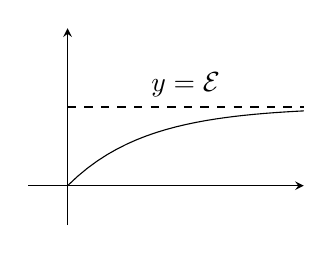
\begin{tikzpicture}
    \draw[-stealth] (-0.5,0) -- (3,0);
    \draw[-stealth] (0,-0.5) -- (0,2);
    \draw[domain=0:3] plot({\x},{(1-e^(-\x))});
    \draw[dashed] (0,1) -- (3,1)
      node[pos=0.5,above]{$y=\mathcal{E}$};
  \end{tikzpicture}
\end{center}
Come notiamo, il grafico tende a raggiungere il valore massimo però senza mai raggiungerlo,
infatti
\begin{equation*}
  \lim\limits_{t\to+\infty}q(t) = \mathcal{E}
\end{equation*}
In ogni caso il condensatore raggiunge una carica quasi totale dopo $4\tau$ o $5\tau$.

\paragraph{Scarica}
La scarica di un condensatore avviene in maniera molto simile alla carica.
\begin{equation*}
  q(t) = C\mathcal{E}e^{-\frac{t}{\tau}}
\end{equation*}
\begin{equation*}
  i(t) = -\frac{\mathcal{E}}{R}e^{-\frac{t}{\tau}}
\end{equation*}
\begin{equation*}
  V(t) = \mathcal{E}e^{-\frac{t}{\tau}}
\end{equation*}

\subsubsection{Circuiti RL}
I circuiti RL sono circuiti composti da una resistenza e un induttore
\begin{center}
  \begin{circuitikz}\ctikzset{bipoles/length=.9cm}
    \draw(0,0) 
    to[battery1] (1,0)
    to[switch] (2,0)
    to[R] (2,1)
    to[L] (1,1)
    to[short] (0,1)
    to[short] (0,0);
  \end{circuitikz}
\end{center}
In una situazione come questa abbiamo come unica incognita variabile è $i(t)$. Per ricavarla 
possiamo risolvere l'equazione differenziale
\begin{equation*}
  \mathcal{E} = L \frac{\dif i}{\dif t}+Ri
\end{equation*}
Se nel circuito RC l'incognita caratteristica è
$q(t)$, in questo è $i(t)$. Se la carica aveva come massimo $C\mathcal{E}$, la corrente ha
come massimo, secondo la legge di Ohm, $\frac{\mathcal{E}}{R}$. Si dimostra che
\begin{equation*}
  i(t) = \frac{\mathcal{E}}{R} \left( 1-e^{-\frac{t}{\tau}} \right)
\end{equation*}
dove $\tau = \frac{L}{R}$ rappresenta la costante di tempo del circuito.\\
Anche in questo caso il grafico della corrente è
\begin{center}
  \begin{tikzpicture}
    \draw[-stealth] (-0.5,0) -- (3,0);
    \draw[-stealth] (0,-0.5) -- (0,2);
    \draw[domain=0:3] plot({\x},{(1-e^(-\x*3))});
    \draw[dashed] (0,1) -- (3,1)
      node[pos=0.5,above]{$y=i$};
  \end{tikzpicture}
\end{center}
capiamo che in teoria la corrente non raggiungerebbe mai il valore di regime, però generalmente
dopo $4\tau$ o $5\tau$ la variazione è talmente minima che gli strumenti non la misurano più.\\
La formula per la scarica invece è la seguente
\begin{equation*}
  i(t) = i_0e^{-\frac{t}{\tau}}
\end{equation*}

\subsubsection{Circuit RLC in serie}
I circuiti RLC sono i più semplici circuiti completi che si studiano in corrente alternata. Essi 
infatti sono come il seguente
\begin{center}
  \begin{circuitikz}\ctikzset{bipoles/length=.9cm}
    \draw(0,0) to[sV] (2,0) 
    to[R] (2,2)
    to[L] (1,2)
    to[C] (0,2)
    to[short] (0,0);
  \end{circuitikz}
\end{center}
Per trovare le formule, dobbiamo introdurre un nuovo concetto, il \textbf{fasore}.
\paragraph{Fasori}
Permettono la trasformazione da funzione sinusoidale a vettore, così da visualizzare lo sfasamento
e i moduli di tutti. La formula generale
\begin{equation*}
  y = A\sin(\omega t+\phi)
\end{equation*}
può essere visualizzata come il seguente vettore
\begin{center}
  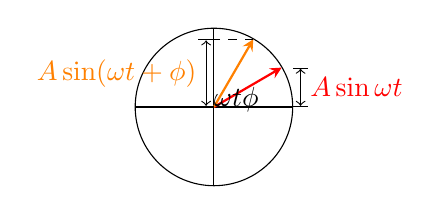
\begin{tikzpicture}
    \draw coordinate (O) (0,0) circle (1);
    \coordinate (A) at (1,0);
    \coordinate (V1) at (0.86,0.5);
    \coordinate (V2) at (0.5,0.86);

    \draw[thin] (-1,0) -- ++(2,0);
    \draw[thin] (0,-1) -- ++(0,2);
    \draw[thick, red, -stealth] (0,0) -- (V1);
    \draw[thick, orange, -stealth] (0,0) -- (V2);
    \draw[thin, dashed] (V2) -- ++(-0.5,0);
    \draw[|<->|] (-0.1,0) -- ++(0,0.86)
      node[orange, pos=0.5, left]{$A\sin(\omega t+\phi)$};
    \draw[|<->|] (1.1,0) -- ++(0,0.5)
      node[red, pos=0.5, right]{$A\sin\omega t$};

    \markangle{O}{A}{V1}{0.5}{1.5}{$\omega t$}
    \markangle[orange]{O}{V1}{V2}{0.7}{1.3}{$\phi$}
  \end{tikzpicture}
\end{center}
Possiamo quindi, per chiarire meglio, rappresentare i circuiti elementari in alternata. Così è
più chiaro vedere i vettori che rappresentano corrente e la forza elettromotrice.
\begin{center}
  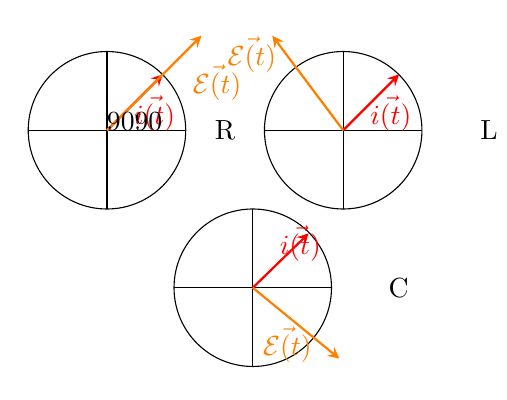
\begin{tikzpicture}
    \draw coordinate (O) (0,0) circle (1);
    \coordinate (A) at (1,0);
    \coordinate (V1) at (0.71,0.71);
    \coordinate (V2) at (1.2,1.2);

    \draw[thin] (-1,0) -- ++(2,0);
    \draw[thin] (0,-1) -- ++(0,2);
    \draw[thick, red, -stealth] (0,0) -- (V1)
      node[pos=0.3, right]{$\vec{i(t)}$};
    \draw[thick, orange, -stealth] (0,0) -- (V2)
      node[pos=0.8, below right]{$\vec{\mathcal{E}(t)}$};
    \node at (1.5,0){R};


    \coordinate (O) at (3,0);
    \draw (O) circle (1);
    \coordinate (A) at (4,0);
    \coordinate (V1) at (3.71,0.71);
    \coordinate (V2) at (2.1,1.2);

    \draw[thin] (2,0) -- ++(2,0);
    \draw[thin] (3,-1) -- ++(0,2);
    \draw[thick, red, -stealth] (O) -- (V1)
      node[pos=0.3, right]{$\vec{i(t)}$};
    \draw[thick, orange, -stealth] (O) -- (V2)
      node[pos=0.8, left]{$\vec{\mathcal{E}(t)}$};
    \markangle{O}{V1}{V2}{0.5}{1.4}{$\ang{90}$}
    \node at (4.5,0){L};

    \coordinate (O) at (1.5,-2);
    \draw (O) circle (1);
    \coordinate (A) at (2.5,-2);
    \coordinate (V1) at (2.21,-1.31);
    \coordinate (V2) at (2.6,-2.9);

    \draw[thin] (0.5,-2) -- ++(2,0);
    \draw[thin] (1.5,-3) -- ++(0,2);
    \draw[thick, red, -stealth] (O) -- (V1)
      node[pos=0.3, above right]{$\vec{i(t)}$};
    \draw[thick, orange, -stealth] (O) -- (V2)
      node[pos=0.8, left]{$\vec{\mathcal{E}(t)}$};
    \markangle{O}{V1}{V2}{0.5}{1.6}{$\ang{90}$}
    \node at (3,-2){C};
  \end{tikzpicture}
\end{center}
Possiamo vedere quindi il rapporto tra corrente e forza elettromotrice.\\ [\baselineskip]
Possiamo usare quindi questa tecnica per vedere come definire la corrente in un circuito LRC. Per
comodità, poniamo la corrente sull'asse delle $x$ così che venga più facile il disegno.
\begin{center}
  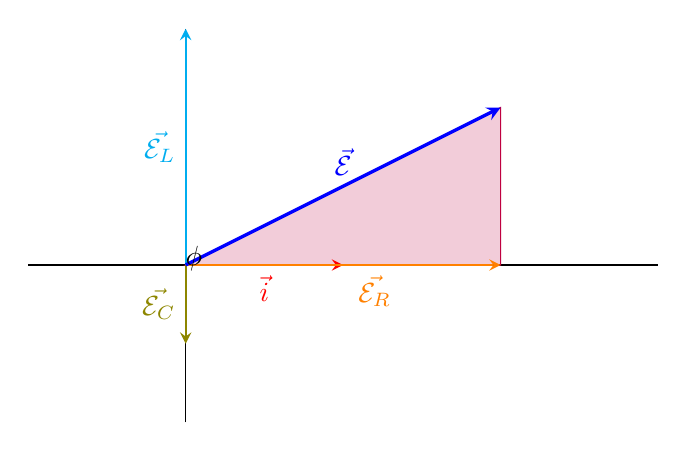
\begin{tikzpicture}
    \coordinate (O) at (0,0);
    \draw[thin] (-2,0) -- ++(8,0);
    \draw[thin] (0,-2) -- ++(0,5);

    \coordinate (i) at (2,0);
    \coordinate (El) at (0,3);
    \coordinate (Ec) at (0,-1);
    \coordinate (Er) at (4,0);
    \coordinate (E) at (4,2);

    \filldraw[purple, fill opacity = 0.2] (O) -- (E) -- (Er) -- cycle;

    \draw[-stealth, thick, red] (O) -- (i)
      node[pos=0.5, below]{$\vec{i}$};
    \draw[-stealth, thick, cyan] (O) -- (El)
      node[pos=0.5, left]{$\vec{\mathcal{E}_L}$};
    \draw[-stealth, thick, olive] (O) -- (Ec)
      node[pos=0.5, left]{$\vec{\mathcal{E}_C}$};
    \draw[-stealth, thick, orange] (O) -- (Er)
      node[pos=0.6, below]{$\vec{\mathcal{E}_R}$};
    \draw[-stealth, very thick, blue] (O) -- (E)
      node[pos=0.5, above]{$\vec{\mathcal{E}}$};

    \markangle{O}{Er}{E}{1}{1.5}{$\phi$}
  \end{tikzpicture}
\end{center}

Per andare a spiegare questo disegno, andiamo a definire alcune delle lettere usate. Essendo in
alternata, sia il condensatore, sia l'induttanza creeranno delle reattanze. Quindi la d.d.p.\ ai
capi dei componenti diventa 
\begin{equation*}
  \mathcal{E}_L = x_L\cdot i_0 \quad \mathcal{E}_C = x_C\cdot i_0 \quad \mathcal{E}_R = R\cdot i_0
\end{equation*}
L'unica incognita che possiamo avere è la corrente $i_0$, quindi dobbiamo trovare il modo per
ricavarla.\\
Secondo la legge di Kirchohoff delle maglie, possiamo dire che
\begin{equation*}
  \vec{\mathcal{E}} = \vec{\mathcal{E}_R} + \vec{\mathcal{E}_L} + \vec{\mathcal{E_C}}
\end{equation*}
Essendo questi dei vettori, possiamo semplicemente fare la somma
vettoriale e quindi andare a calcolare l'ipotenusa del triangolo evidenziato.
\begin{align*}
  \mathcal{E}^2 &= R^2i_0^2+(x_L-x_C)^2i_0^2\\
  \mathcal{E}^2 &= i_0^2[R^2+(x_L-x_C)^2]\\
  i_0 &= \frac{\mathcal{E}_0}{\sqrt{R^2+(x_L-x_C)^2}}
\end{align*}
Questo porta alla definizione della legge per la corrente
Viene definita \textbf{impedenza}
\begin{equation*}
  Z = \sqrt{R^2+(x_L-x_C)^2} 
\end{equation*}
\begin{equation*}
  i(t) = \frac{\mathcal{E}_0}{Z}\sin \left( \omega t+\phi \right)
\end{equation*}
L'unica cosa che manca da trovare è $\phi$, lo sfasamento. Nel disegno è già evidenziato ed è
evidente che non è altro se non un angolo tra due vettori, quindi si deduce che
\begin{equation*}
  \phi = \arctan \left( \frac{x_L-x_C}{R} \right)
\end{equation*}
Quale deve essere la frequenza del generatore perché la reattanza 
capacitiva e quella induttiva si equivalgano? In altri termini, quando possiamo semplificare
il circuito in modo che abbia solo la resistenza? Nella \textbf{condizione di risonanza}
la frequenza è pari a
\begin{equation*}
  f = \frac{1}{2\pi\sqrt{LC}}
\end{equation*}

\subsection{Leggi di Kirchhoff}
Per capire queste leggi, è necessario aver chiaro tre termini
\begin{description}
  \item[Nodo] Un punto in cui convergono almeno 3 conduttori
  \item[Ramo] Una parte di circuito tra 2 nodi
  \item[Maglia] Una parte di circuito attraversata solo una volta per tornare al nodo di origine
\end{description}
Per spiegarli, prendiamo il seguente circuito
\begin{center}
  \begin{circuitikz}\ctikzset{bipoles/length=.8cm}
    \draw (0,0) 
    to[short] (1,0)
    to[R,-o](2,0)
    to[short] (3,0)
    to[battery1] (3,-1)
    to[short] (3,-2)
    to[short,-o] (2,-2)
    to[short](0,-2)
    to[battery1](0,-1)
    to[short](0,0);
    \draw (2,0)
    to[R] (2,-2);
  \end{circuitikz}
\end{center}
Vediamo due nodi (già evidenziati dai cerchi). Sono presenti 3 rami (tutti i modi per arrivare
da un nodo all'altro) e 3 maglie (la maglia sinistra con 2 resistenze e una batteria, quella destra
con una sola resistenza e una batteria e quella che comprende i rami esterni).\\
Una caratteristica da ricordare è che \emph{ci sono tante correnti quanti rami}. Risolvere questi
circuiti quindi significa trovare intensità e verso di queste correnti.

\subsubsection{Legge di Kirchhoff dei nodi}
La corrente entrante in un nodo è pari a quella uscente.
\begin{equation*}
  \sum_k i_k = 0
\end{equation*}
Questo è anche definito come \textbf{Principio di conservazione di carica}.

\subsubsection{Legge di Kirchhoff delle maglie}
Per arrivare alla formula, prendiamo come esempio il seguente circuito
\begin{center}
  \begin{circuitikz}\ctikzset{bipoles/length=.8cm}
    \draw (0,0)
    to[battery1, l = $\mathcal{E}_1$] (0,-1)
    to[R = $R_1$,i<_=$i_1$] (0,-2)
    to[R = $R_2$,i<_=$i_2$] (4,-2)
    to[R = $R_3$,i<_=$i_3$] (4,-1)
    to[battery1, l = $\mathcal{E}_2$] (4,0)
    to[battery1, l = $\mathcal{E}_3$] (2,0)
    to[R = $R_4$,i<_=$i_4$] (1,0)
    to (0,0);

    \draw[-stealth] (2,-0.5) arc(-260:70:0.4); 
  \end{circuitikz}
\end{center}
Kirchhoff descrive che
\begin{equation*}
  \sum_k \mathcal{E}_k = \sum_j R_ji_j
\end{equation*}
Ovvero scegliendo un verso (orario o antiorario) se la corrente ha stesso verso le si da il valore $+$,
altrimenti $-$. Stessa cosa per la forza elettromotrice. Proseguendo da un nodo qualsiasi secondo il
verso scelto e tornando sullo stesso nodo (attraversando una maglia), sommiamo algebricamente le
forze o le resistenze che si incontrano. Si ottiene quindi la formula descritta.

\subsubsection{Utilizzo delle leggi di Kirchhoff}
Negli esercizi non possiamo usare direttamente queste leggi. Il modo generale di approcciarsi è
\begin{enumerate}
  \item Individuare le incognite (le correnti) e scegliere un verso di percorrenza in modo arbitrario
  \item Creare un sistema a $n$-equazioni dove $n$ è il numero di incognite (in generale 3)
  \item Come prima equazione, usare la Legge di Kirchhoff dei Nodi scegliendo arbitrariamente
    i versi delle correnti nel nodo
  \item Come seconda e terza equazione, descrivere le maglie seguendo il verso scelto
  \item Risolvere il sistema lineare. Nel caso in cui una corrente sia negativa, il suo risultato
    è $\abs{i}$.
\end{enumerate}

\subsection{Mutua induzione}
La mutua induzione è il fenomeno dell'induzione che avviente tra due o più circuiti diversi. Ad
esempio se un circuito $1$ agisce su di un circuito $2$,
\begin{equation*}
  \Phi_2(\vec{B}) = Mi_2
\end{equation*}
dove $M$ è un valore che varia da circuito a circuito.\\
Si noti che di conseguenza, per la legge di Faraday-Neuman-Lenz, si genererà una forza 
elettromotrice da un circuito all'altro. Quindi possiamo scrivere
\begin{equation*}
  \mathcal{E}^{1\to2}= - M \frac{\dif i}{\dif t}
\end{equation*}


\subsection{Corrente Alternata}
Se fin'ora si è lavorato con corrente continua fornita da una forza elettromotrice, quasi tutta
la corrente che si utilizza quotidianamente è alternata. Per generare corrente alternata, si
pongano due magneti con polarità opposte uno di fronte all'altro. Tra i due si ponga una serie
di spire che ruotano. Questa rotazione genererà una corrente. Il disegno dunque è molto simile
a quello del motore elettrico
\begin{center}
  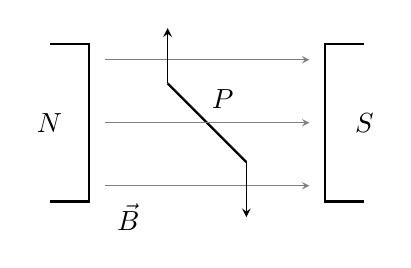
\begin{tikzpicture}
    % Magnets
    \coordinate (N1) at (0,1);
    \coordinate (N2) at (0,-1);
    \coordinate (S1) at (3,1);
    \coordinate (S2) at (3,-1);
    % Plate
    \coordinate (P1) at (1,0.5);
    \coordinate (P2) at (2,-0.5);

    % Magnets
    \draw[thick] (-0.5,1) -- (N1) -- (N2) -- (-0.5,-1);
    \draw[thick] (3.5,1) -- (S1) -- (S2) -- (3.5,-1);
    % Plate
    \draw[thick] (P1) -- (P2);

    % Magnetic lines
    \foreach \a in {0.8,0,-0.8}{
      \draw[gray, very thin, -stealth] (0.2, \a) -- ++(2.6,0);
    }

    \draw[-stealth] (P1) -- ++(0,0.7);
    \draw[-stealth] (P2) -- ++(0,-0.7);

    % Annotations
    \node at (-0.5,0){$N$};
    \node at (3.5,0){$S$};
    \node at (1.7,0.3){$P$};
    \node at (0.5,-1.2){$\vec{B}$};
  \end{tikzpicture}
\end{center}
Facendo girare le spire, il flusso varierà. Infatti si avrà
\begin{equation*}
  \Phi(\vec{B})=BS\cos\theta = BS\cos\omega t
\end{equation*}
quindi applicando la legge di Faraday-Neuman-Lenz
\begin{align*}
  &\mathcal{E} = -\frac{\dif\Phi(\vec{B})}{\dif t} = -\frac{\dif}{\dif t}[BS\cos\omega t] =\\
  &-BS \frac{\dif}{\dif t}[\cos\omega t]=\omega BS\sin\omega t= \mathcal{E}_0\sin\omega t 
\end{align*}
Notiamo quindi che la forza elettromotrice che viene scaturita ha intensità sinusoidale, quindi
lo è anche la corrente. Infatti si definisce una funzione $i(t)$ che varia a seconda del tempo
\begin{equation*}
  i(t) = \frac{\mathcal{E}}{R}\sin\omega t = i_0\sin\omega t
\end{equation*}
dove $i_0$ è il valore di picco. Si definisce anche una corrente efficace $i_{eff}$ che è la
corrente che dissipa la stessa potenza in corrente continua. Il suo valore è
\begin{equation*}
  i_{eff} = \frac{i_0}{\sqrt{2}}
\end{equation*}
Quindi in generale
\begin{equation*}
  \mathcal{E} = R\cdot i(t)\quad\mathcal{E}_0=R\cdot i_0\quad\mathcal{E}_{eff}=R\cdot i_{eff}=
  \frac{\mathcal{E}_0}{\sqrt{2}}
\end{equation*}
Si introduce anche un nuovo elemento circuitale il generatore di corrente alternata
\begin{center}
  \begin{circuitikz}
    \draw (0,0) to[short] (1,0) to[sV] (2,0) to[short] (3,0);
  \end{circuitikz}
\end{center}

\subsection{Trasformatore}
Il trasformatore è uno dei dispositivi più usati al mondo. Il suo scopo è quello di 
\emph{trasformare} un voltaggio in uno maggiore o minore, quasi senza perdita di energia. Di 
seguito verrà schematizzato il trasformatore
\begin{center}
  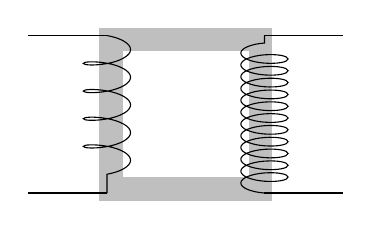
\begin{tikzpicture}
    \fill[fill=gray!50] (-0.1,1.1) -- ++(2.2,0) -- ++(0,-0.3) -- ++(-2.2,0) -- cycle;
    \fill[fill=gray!50] (-0.1,-0.8) -- ++(2.2,0) -- ++(0,-0.3) -- ++(-2.2,0) -- cycle;
    \fill[fill=gray!50] (-0.1,0.8) -- ++(0.3,0) -- ++(0,-1.6) -- ++(-0.3,0) -- cycle;
    \fill[fill=gray!50] (1.8,0.8) -- ++(0.3,0) -- ++(0,-1.6) -- ++(-0.3,0) -- cycle;
    \draw[decoration={aspect=0.3, amplitude=3mm,coil}, decorate] (0,1) -- (0,-1);
    \draw (-1,1) -- (0,1);
    \draw (-1,-1) -- (0,-1);
    \draw[
      rotate around={180:(2,0)},decoration={
        aspect=0.3, amplitude=3mm, segment length=1.5mm,coil
      }, decorate]
      (2,1) -- (2,-1);
    \draw (3,1) -- (2,1);
    \draw (3,-1) -- (2,-1);
  \end{tikzpicture}
\end{center}
Sia la spira di sinistra quella \textbf{primaria} e sia quella di destra la \textbf{secondaria}.
Perché un trasformatore abbia senso di esistere deve avere un numero diverso di spire a destra
e a sinistra. Il blocco di ferro-metallo al centro serve ad incanalare tutte le linee di forza, 
così che non si sprechino. Si trovano le seguenti formule
\begin{equation*}
  \frac{\mathcal{E}_p}{\mathcal{E}_s} = \frac{n_p}{n_s} = \frac{i_s}{i_p}
\end{equation*}
Si presti attenzione alla sequenza di scrittura.
Si noti anche che $\frac{n_s}{n_p}$ è definito \emph{rapporto di trasformazione}.
